\documentclass[journal]{IEEEtran}
\usepackage{amsmath,amssymb,amsfonts}
\usepackage{graphicx}
\usepackage{cite}
\usepackage{booktabs}
\usepackage{caption}
\usepackage{array}
\usepackage{float}
\usepackage{pdflscape}

% pandoc writeup.md --template=mytemplate.tex -o output.pdf --bibliography=refs.bib --pdf-engine=pdflatex --citeproc --csl=ieee.csl



\title{Lite Learning: Efficient Crop Classification in Tanzania Using Traditional Machine Learning \& Crowd Sourcing}

\author{
    Michael L. Mann, 
    Lisa Colson,
    Rory Nealon,
    Ryan Engstrom,
    Stellamaris Nakacwa
    \thanks{Michael L. Mann and Ryan Engstrom are with The George Washington University, Washington DC 20052 (e-mail: mmann1123@gmail.com).}
    \thanks{Lisa Colson is with the USDA Foreign Agricultural Service, Washington DC 20250.}
    \thanks{Rory Nealon is with USAID GeoCenter, Washington DC 20523.}
    \thanks{Stellamaris Nakacwa is with YouthMappers, Texas Tech University, Lubbock TX 79409.}
}

\begin{document}

\maketitle

\begin{abstract}
This study introduces a novel approach to traditional machine learning methodology for crop type classification in Tanzania, by integrating crowdsourced data with time-series features extracted from Sentinel-2 satellite imagery. Leveraging the YouthMappers network, we collected ground validation data on various crops, including challenging types such as cassava, millet, sunflower, sorghum, and cotton across a range of agricultural areas. Traditional machine learning algorithms, augmented with carefully engineered time-series features, were employed to map the different crop classes. Our approach achieved high classification accuracy, evidenced by a Cohen's Kappa score of 0.82 and an F1-micro score of 0.85. The model often match or outperform broadly used land cover models which simply classify 'agriculture' without specifying crop types. By interpreting feature importance using SHAP values, we identified key time-series features driving the model's performance, enhancing both interpretability and reliability. Our findings demonstrate that traditional machine learning techniques, combined with computationally efficient feature extraction methods, offer a practical and effective “lite learning” approach for mapping crop types in data-scarce environments. This methodology facilitates accurate crop type classification using a low-cost, resource-limited approach that contributes valuable insights for sustainable agricultural practices and informed policy-making, ultimately impacting food security and land management in resource-limited contexts, such as sub-Saharan Africa.
\end{abstract}

\begin{IEEEkeywords}
Remote sensing, machine learning, crop classification, time-series analysis, crowdsourcing, Sentinel-2, feature engineering.
\end{IEEEkeywords}

\section{Introduction}
\subsection{Background and Context}

The free access to remotely sensed data, such as imagery from satellites (e.g. Sentinel-2, Landsat), has allowed for crop type classification in developing countries. By leveraging the power of advanced imaging technologies combined with machine learning algorithms, researchers and practitioners can now identify and map different crop types over large geographic areas at no or low cost \cite{hersh2021open}. This has the potential to improve food security, land use planning, and agricultural policy in regions where ground-based data collection is limited or non-existent \cite{rs10010099, li2023development, ibrahim2021mapping}.

In recent years, machine learning approaches have emerged as powerful tools for crop type classification using remotely sensed data. Specifically, methods based on machine learning algorithms have gained recognition for their effectiveness in matching valuable spectral information from satellite imagery to observations of crop type for particular locations. Machine learning algorithms, including decision trees, random forests, support vector machines (SVM), and k-nearest neighbors (KNN), have been successfully used to  classify imagery into unique agricultural types \cite{@ibrahim2021mapping, begue2018remote, delince2017handbook}. These algorithms leverage the rich spectral information captured by satellite sensors, allowing them to identify distinctive patterns associated with different crop types. By training on large labeled datasets where ground-validation information on crop types is linked to corresponding image pixels, these models can effectively learn the relationships between the spectral characteristics of crops and their respective classes \cite{rs10010099}.

The strength of traditional machine learning approaches lies in their ability to exploit both the spectral and time-series patterns within the remotely sensed data. Traditional machine learning approaches offer advantages in terms of interpretability and computational efficiency compared to deep learning architectures. They provide insight into the decision-making process and can be more readily understood and explained by domain experts. Additionally, these methods are generally less computationally demanding and require less training data, making them suitable for applications with limited computational resources \cite{hohl2024recent, rs13132591, agriculture13050965, LI2023103345, MA2019166}.
 

Traditional machine learning algorithms require the extraction of variables (e.g. max EVI, mean blue band) that can help distinguish different plant or crop types \cite{begue2018remote}. The development of salient time-series features to capture phenological differences between locations from remotely sensed images remains a challenge. These features are typically derived from the spectral bands (e.g. red edge, NIR) of the satellite imagery or indexes, such as the enhanced vegetation index (EVI), and basic time series statistics (e.g. mean, max, minimum, slope) for the growing season \cite{morton2006cropland}. Meanwhile a broader set of time series statistics from bands or indexes may be more relevant for a number of applications. For instance the skewness of EVI might help distinguish crops that green-up earlier vs later in the season, measures of the numbers of peaks in EVI might help differentiate intercropping or multiple plantings in a season \cite{begue2018remote}. However, the selection and extraction of these features can be time-consuming and labor-intensive, requiring domain expertise and manual intervention.

In contrast, deep learning methods have dominated the most recent literature \cite{agriculture13050965, @hohl2024recent}. These methods include both recurrent neural networks (RNN) and convolutional neural networks (CNN). Recurrent Neural Networks (RNNs) are a class of neural networks that are particularly powerful for modeling sequential data such as time series, speech, text, and audio. The fundamental feature of RNNs is their ability to maintain a 'memory' of previous inputs by using their internal state (hidden layers), which allows them to exhibit dynamic temporal behavior. RNNs and its variants allow the integration of time-series imagery, significantly improving crop type classification outcomes especially in data rich environments \cite{agriculture13050965, camps2021deep}. Deep learning approaches however typically require much larger sets of training data, may be more prone to overfitting especially with small sample sizes, have significant limitations to interpretability, and require expensive compute \cite{hohl2024recent, rs13132591, agriculture13050965, LI2023103345, MA2019166}. Although recent efforts have closed the gap e.g. \cite{tseng2021cropharvest}, the lack of readily available and reliable ground truth data or benchmark datasets for training, as discussed earlier, may limit the applicability of deep learning for a variety of tasks including crop classification and make researchers more reliant of less reliable techniques like transfer learning or zero-shot or low shot methods \cite{owusu2024towards, LI2023103345, MA2019166}. Moreover, training data for extreme events, like crop losses, disease, and lodging are largely non-existant.  Interpretability is also a salient weakness as interpretation of models allows us to gain scientific insight and assess trustworthiness and fairness in so far as outputs affect policy decisions.  

% An alternative approach turns back the clock on deep learning approaches. For instance CNN classifiers, through the exertion of tremendous effort of GPUs, can apply and learn from thousands of filters or convolutions that help detect distinct features like edges, textures or patterns. It is however possible to apply a more limited yet salient set of filters like Fourier Transforms, Differential Morphological Profiles [@pesaresi2001new], Line Support Regions or Structural Feature Sets [@huang2007classification] amongst others, to images and then use these as features in more traditional machine learning approaches [@graesser2012image, @owusu2024towards, @engstrom2022poverty; @chao2021evaluating; @urbansci7040116]. This approach may be particularly useful in data-scarce environments, requiring less training data and potentially offering more efficient results in low-information settings. The same approach has been taken for time series analysis, where instead of learning patterns through a RNNs memory, we can apply a more limited but potentially salient series of time series filters. Measures of trends, descriptions of distributions, or measures of change and complexity might adequately describe time series properties for regression and classification tasks [@christ2018time; @yang2021anomaly]. This time series filter approach, developed for this paper, can also be applied on a pixel-by-pixel basis to satellite image bands or index values[@xr_fresh_2021].

% Field-collected data provides the necessary validation and calibration for remote sensing-based models. It serves as the benchmark against which the model's predictions are evaluated and refined. Ground validation data collected through field visits, observation, and interactions with local farmers offers essential insights into the specific crop types present in the study area. Validating and training models with accurate ground reference information allows for the spectral patterns captured by remote sensing data to be correctly associated with the corresponding crop. By combining the spectral information from satellite imagery with ground validation data, researchers can develop robust models that effectively differentiate between different crop types based on their unique spectral signatures and temporal patterns.

% The collection of field observations and ground validation data is a critical input for the development of models to classify crop types [@delince2017handbook; @MA2019166]. However, obtaining accurate and timely ground validation data can be challenging in developing countries due to limited resources, infrastructure, and local capacity [@delince2017handbook; @begue2018remote]. In many cases, researchers rely on crowdsourced data from volunteers or citizen scientists to supplement or validate ground truth data collected through traditional methods. Projects like [@tseng2021cropharvest] point to the paucity of multi-class crop type datasets globally. This is a significant gap in the field of crop type classification, as the availability of high-quality training data is essential for the development of accurate and reliable machine learning models [@rs13132591].
 

% In this study we aim to address two critical challenges in the field of crop type classification: the lack of in-season multi-class crop type datasets, and the need for new methods to obtain high accuracy crop type predictions from limited amounts of training data.
 
% We propose a novel approach that combines crowdsourced data with a new automated approach to extracting time-series features from satellite imagery. We apply this new approach to classify crop types in Northern Tanzania. By leveraging the power of crowdsourcing and remote sensing technologies, we aim to develop a robust and scalable solution for crop type classification that can be adapted to other regions and contexts with a minimal or no cost.
 


\section{Methodology}
\subsection{Study Area}
 
\subsection{Data Collection}
 

\subsection{Satellite Imagery and Preprocessing}
 
\subsection{Feature Engineering}
Using the \texttt{xr\_fresh} toolkit, we computed time-series statistics, including absolute energy, autocorrelation, skewness, and variance. These features enhance the interpretability and efficiency of traditional machine learning classifiers.

\subsection{Model Selection and Evaluation}
Optuna was employed for hyperparameter tuning across multiple classifiers, including LightGBM and Random Forest. Model performance was assessed using stratified group k-fold cross-validation, ensuring robustness against data leakage. SHAP values provided insights into feature importance.

\section{Results and Discussion}
The model achieved an overall accuracy of 85\%, with particularly strong performance for maize and rice classification. SHAP-based feature analysis revealed that SWIR bands and vegetation indices played a critical role in distinguishing crop types.

\begin{figure}[H]
    \centering
    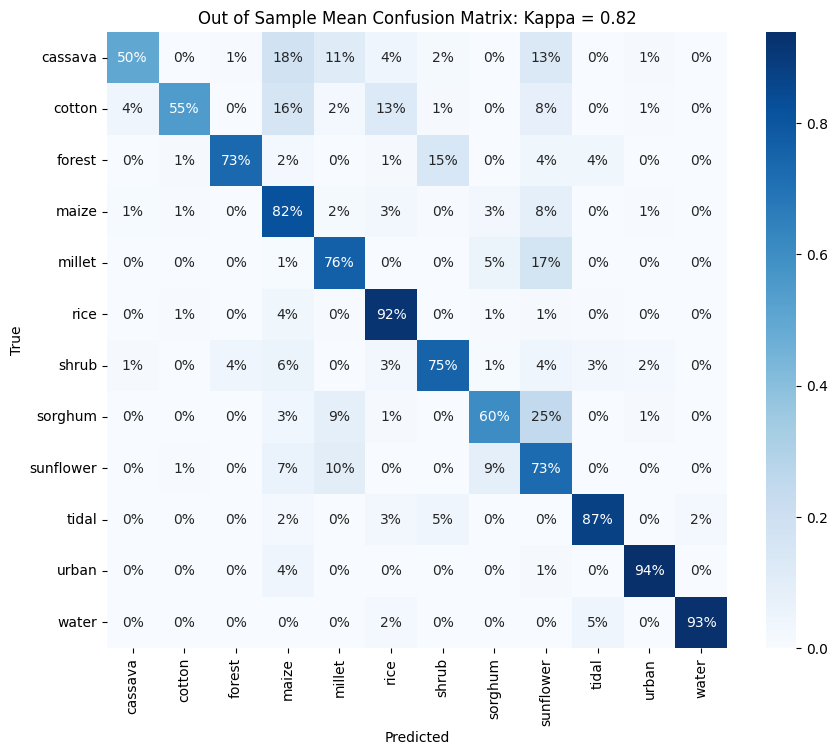
\includegraphics[width=0.8\linewidth]{/home/mmann1123/Documents/github/YM_TZ_crop_classifier/writeup/figures/final_confusion_no_other_model_selection_feature_selection_no_otherLGBM_kappa_3.png}
    \caption{Confusion Matrix of Crop Classification Model}
    \label{fig:confusion}
\end{figure}

\section{Conclusion}
This study demonstrates that traditional machine learning methods, when combined with engineered time-series features, offer an interpretable and computationally efficient solution for crop classification in Tanzania. Future work should explore integrating additional spectral indices and expanding the dataset for improved model generalizability.

\bibliographystyle{IEEEtran}
\bibliography{/home/mmann1123/Documents/github/YM_TZ_crop_classifier/writeup/refs.bib}

\end{document}
